%===================================== CHAP 4 =================================

\chapter{Method and calculations}

Simulated experiments with two neurons and one directed synaptic connection was performed for test purposes. Various approaches for inferring time varying weighs was tried and their limitations were investigated.  the ability of the method to infer time varying weights and to investigate its limitations. In section \ref{Method} the method of the test experiments is described in detail. Section \ref{Precalc} presents some calculations based on probability theory to show how well we can expect the method to perform.

\subsection{Background from Linderman's work}
\label{Linderman}

\subsection{Method}
\label{Method}

In this project the test case is a simple model with two neurons, 1 and 2, and a synaptic weight, $w_{12}$ directed from neuron 1 to neuron 2.

\begin{figure}[h]
    \centering
    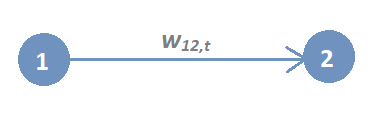
\includegraphics[scale=0.6]{Two_neurons_illustration.png}
\end{figure}

$N_1$ has for each time step a constant probability for spiking that depends on some background rate $b_1$. $N_2$ has spiking probability that depends on the spiking of $N_1$ in the previous time step through the linear predictor $b_2 + w_{21,t} \cdot s_{1,t-1}$. 

\begin{align*}
    s_{1t} \sim \text{Ber}(\pi_{1t}) && \pi_{1t}= \frac{1}{1+e^{-b_1}} \\
    s_{2t} \sim \text{Ber}(\pi_{2t}) && \pi_{2t}= \frac{1}{1+e^{-(b_2 + w_{21,t} \cdot s_{1,t-1})}}
\end{align*}

For the test cases the parameter values to be used are $b1 = 0.5$ and $b2 = 0$. This corresponds to a background firing rate of 0.62 and 0.5 for neuron 1 and 2 respectively. The value for the weight $w_{12}$ will be let to vary with time, but a typical size for it will be $w_{12}=0.7$. This gives a value of 1.2 for the linear predictor when neuron 1 spiked in the previous time step, and a corresponding firing rate of 0.77 for neuron 2. This is summed up in table 

\begin{center}
 \begin{tabular}{||c c c c||} 
 \hline
 Neuron & b & \pi_{s_{1,t-1}=0} & \pi_{s_{1,t-1}=1} \\ [0.5ex] 
 \hline\hline
 1 & 0.5 & 0.62 & 0.62 \\ 
 \hline
 2 & 0  & 0.5 & 0.77 \\
 [1ex] 
 \hline
\end{tabular}
\end{center}

\begin{itemize}
    \item Write the things I do in the coding that is necessary to understand what I have done and to reproduce my work.
\end{itemize}


\subsection{Precalculations}
\label{Precalc}

\begin{itemize}
    \item The aim here is to calculate how well I expect my tests to work. Can use hypothesis testing on bernoulli GLM 
    \item Say something about how many time points ect that is needed to be able to detect a change of the weights
\end{itemize}

\begin{wraptable}{r}{4cm}
\begin{center}
 \begin{tabular}{||c c c ||} 
 \hline
 n & Lower & Upper \\ [0.5ex] 
 \hline\hline
 10 & 0.5 & 1 \\ 
 \hline
 100 & 0.7 & 0.84 \\
 \hline
 1000 & 0.748 & 0.792 \\
 \hline
 10000 & 0.7631 & 0.7769 \\ [1ex] 
 \hline
\end{tabular}
\end{center}
\end{wraptable}

\begin{figure}[h]
    \centering
    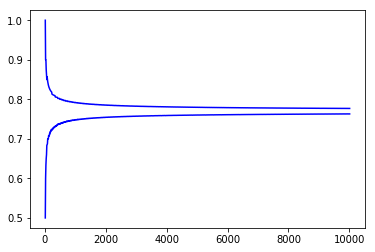
\includegraphics[scale=0.7]{Conf_intervals.png}
\end{figure}

It is practical to have some understanding of how precisely the weights can be inferred from the spike data. When performing $n$ repeated trials of a Bernoulli process with success rate $\pi$, the sum successes comes from a binomial distribution, with parameters $n$ and $\pi$. For some success count, $n_{success}$, the parameter $\pi$ can be estimated as $\frac{n_{success}}{n}$. How good this estimate is depends on the number of trials, $n$. Figure ?? and table ?? presents the endpoints of range that contains 90\% of the distribution, for different values of n (scaled by one over n). 